% Generated by scripts/make_paper_tables.py -- do not edit by hand.
\section{Results}\label{sec:results}
Unless noted, results are averages over the 17 decontaminated tasks and five seeds.

\paragraph{Noise floors.} Table~\ref{tab:ceil} lists the estimates. $\mathrm{RMSE}_{\mathrm{floor}}$ ranges from 0.31 to 0.79 pChEMBL units and $R^2_{\max}$ from 0.56 to 0.96. The median $\hat s$ is 0.47 for $K_i$ tasks and 0.66 for $\mathrm{IC}_{50}$ tasks, of the same order as earlier ChEMBL-wide estimates for $K_i$ (0.54)~\cite{kramer2012experimental} and the reported 25\% larger spread of $\mathrm{IC}_{50}$ data~\cite{kalliokoski2013comparability}; in our set the measurement type is confounded with target class ($K_i$ tasks are mostly GPCRs, $\mathrm{IC}_{50}$ tasks mostly kinases), so we do not attribute the difference to the measurement type. Replicates are often concentrated in few document pairs: CHEMBL237\_IC50 rests on 7 document pairs, one of which contributes 79\% of molecule pairs. Accordingly, the bootstrap over document pairs gives intervals more than 20\% wider than the bootstrap over molecules for 9 of 17 tasks, and 4 and 5 times as wide for CHEMBL237\_IC50 and CHEMBL2971\_IC50 (for the latter, 0.53--1.15); it is narrower only for tasks with many document pairs. Table~\ref{tab:robust} shows the sensitivity to curation: counting identical values from different documents once raises $\hat s$ by up to 0.14 (CHEMBL237\_Ki), and a stereo-aware molecule definition changes it by more than 0.05 for 7 tasks. These are the uncertainties of the reference point against which all models below are scored.

\paragraph{Fraction of ceiling.} Table~\ref{tab:frac} gives mean $f$ by model and split. ECFP+RF is the best model on every split. On random splits its mean $f$ is 0.90, but the median is 0.82, the mean without the tasks where it exceeds 1 is 0.80, and computing the floor at the ends of the confidence interval of $\hat s$ moves the mean between 0.80 and 1.03. On scaffold and temporal splits the means are 0.73 and 0.36 (medians 0.68 and 0.34). Thus most of the reducible error is captured on random splits, whereas on temporal splits about two thirds of it remains; improvements are measurable mainly on the harder splits.

\paragraph{ECFP versus frozen embeddings.} Frozen ChemBERTa-77M and MoLFormer-XL-10\% embeddings with a GBM head are below ECFP+GBM on every split (Table~\ref{tab:paired}, Figure~\ref{fig:paired}): by 0.16--0.22 in $f$ on random and scaffold splits, where they are worse on all 17 tasks, and by 0.07 on temporal splits, where they are better on only 3--4 of 17 tasks (Holm-adjusted $p\le0.033$ in all cases). ECFP+RF is slightly better than ECFP+GBM (0.02--0.03 in $f$; better on 13 of 17 tasks). In a three-task pilot (CHEMBL237\_IC50, CHEMBL206\_IC50, CHEMBL204\_Ki) frozen embeddings had appeared better than ECFP on temporal splits; on 17 tasks this did not hold. The conclusion concerns two small frozen models with a tree-based head, not pretrained models in general.

\paragraph{D-MPNN and fine-tuning.} Table~\ref{tab:subset} compares all models on the 5 tasks where the D-MPNN and fine-tuned ChemBERTa were run. On random and scaffold splits neither reaches ECFP, and fine-tuning does not improve on the frozen embedding. On temporal splits the fine-tuned model has the highest mean (0.31 versus 0.28 for ECFP+RF), but this comes from a single task, CHEMBL237\_IC50 (0.48 versus 0.08); on the other 4 tasks the means are 0.27 and 0.33. With 5 tasks we do not test these differences.

\paragraph{Models below the noise floor.} On 5 task--split combinations ECFP+RF scores $f>1$, i.e.\ its test RMSE is below the estimated floor: CHEMBL205\_Ki (random), CHEMBL279\_IC50 (random), CHEMBL2971\_IC50 (random), CHEMBL2971\_IC50 (scaffold), CHEMBL325\_IC50 (random) (Figure~\ref{fig:floor}). These tasks are among those with the largest estimated floors (0.67--0.79), and all but one are random splits. If between-document noise were independent of what a model can learn, this would be impossible in expectation~\cite{kolmar2021noise}; models reaching or exceeding noise-based bounds were also reported by Crusius et al.~\cite{crusius2025fitting}. Two explanations are possible. (i) The floor is over-estimated for these tasks: it is based on molecules that are not representative of the test set, and for CHEMBL2971\_IC50 its interval over document pairs is very wide (0.53--1.15), and two of its document pairs differ by a nearly constant 2.4 and 3.0 log units (standard deviations 0.41 and 0.13 over 29 and 26 shared molecules), which suggests unit errors that the 3-unit trimming does not remove. (ii) Under random splits, molecules from the same document share assay-specific offsets that a model can learn from their neighbours in the training set, so part of the between-document ``noise'' is predictable; models are known to exploit publication-level signals in ChEMBL~\cite{blevins2025cleverhans}. CHEMBL2971\_IC50 also exceeds 1 on the scaffold split, which (ii) explains less easily. A document-grouped split would separate the two explanations and is left for the next version. In either case $f>1$ signals a problem with the floor or the split, not accuracy beyond the measurement limit.

\paragraph{Effect of decontamination.} Repeating the runs on the uncleaned data (Table~\ref{tab:leak}) changes the mean test RMSE by at most 0.006 pChEMBL units for ECFP+GBM, ECFP+RF and the embedding models, and by up to 0.025 for the unstable ECFP+MLP. Mean $f$ is 0.02 higher on the uncleaned data for the former models, mostly because the floors are slightly larger there (by 0.023 on average), not because the errors are smaller. Removing molecules that occur in MoleculeNet or TDC therefore has little effect on these tasks, and the model ranking is unchanged. This is not a pure leakage test: the uncleaned test sets contain 6.7\% more molecules, decontamination removed 24\% of the replicated molecules, and overlap with pretraining corpora is not covered.

\paragraph{Minimum detectable effect.} The median single-test-set MDE for a paired comparison with ECFP+GBM is 0.040, 0.042 and 0.045 in $f$ for ECFP+RF on random, scaffold and temporal splits, and about 0.08 for the embedding models, whose errors are less correlated with the baseline. These values assume independent test molecules and are therefore optimistic. The ECFP+RF advantage is below the MDE of a single test set and is detectable only when pooled over tasks, while the embedding gaps on random and scaffold splits are two to three times the MDE.

\begin{table}[ht]\centering\footnotesize\setlength{\tabcolsep}{4pt}\caption{Noise floors per task (decontaminated data). $n_{\text{rep}}$: replicated molecules after trimming; doc.\ pairs: distinct pairs of documents among the replicates; top \%: share of molecule pairs from the most frequent document pair. 95\% intervals for $\hat s$ from a bootstrap over molecules and over document pairs (1{,}000 resamples); the latter is for the pairwise form of the estimator, which differs slightly from $\hat s$ when molecules have more than two documents. $\mathrm{RMSE}_{\mathrm{floor}}$ and $R^2_{\max}$ over all molecules of the task.}\label{tab:ceil}
\begin{tabular}{lrrrccccc}\toprule Task & $n_{\text{rep}}$ & doc.\ pairs & top \% & $\hat s$ & CI molecules & CI doc.\ pairs & $\mathrm{RMSE}_{\mathrm{floor}}$ & $R^2_{\max}$\\\midrule
CHEMBL203\_IC50 & 396 & 432 & 17 & 0.66 & [0.61, 0.70] & [0.61, 0.71] & 0.65 & 0.75\\
CHEMBL204\_Ki & 133 & 108 & 8 & 0.31 & [0.19, 0.43] & [0.24, 0.44] & 0.31 & 0.96\\
CHEMBL205\_Ki & 156 & 117 & 6 & 0.70 & [0.62, 0.78] & [0.63, 0.82] & 0.70 & 0.62\\
CHEMBL206\_IC50 & 132 & 103 & 13 & 0.53 & [0.42, 0.63] & [0.43, 0.70] & 0.52 & 0.85\\
CHEMBL214\_Ki & 147 & 79 & 11 & 0.49 & [0.41, 0.57] & [0.43, 0.64] & 0.49 & 0.82\\
CHEMBL217\_Ki & 185 & 157 & 7 & 0.44 & [0.38, 0.49] & [0.41, 0.53] & 0.44 & 0.80\\
CHEMBL233\_Ki & 155 & 404 & 2 & 0.55 & [0.44, 0.63] & [0.58, 0.69] & 0.54 & 0.81\\
CHEMBL234\_Ki & 127 & 176 & 5 & 0.42 & [0.35, 0.49] & [0.38, 0.51] & 0.42 & 0.89\\
CHEMBL237\_IC50 & 111 & 7 & 79 & 0.69 & [0.66, 0.74] & [0.51, 0.83] & 0.67 & 0.63\\
CHEMBL237\_Ki & 131 & 105 & 7 & 0.54 & [0.42, 0.64] & [0.46, 0.69] & 0.53 & 0.84\\
CHEMBL251\_Ki & 106 & 97 & 9 & 0.44 & [0.36, 0.52] & [0.36, 0.51] & 0.44 & 0.86\\
CHEMBL279\_IC50 & 229 & 312 & 14 & 0.70 & [0.64, 0.77] & [0.59, 0.80] & 0.70 & 0.61\\
CHEMBL2971\_IC50 & 526 & 153 & 35 & 0.80 & [0.74, 0.86] & [0.53, 1.15] & 0.79 & 0.56\\
CHEMBL325\_IC50 & 218 & 264 & 3 & 0.67 & [0.59, 0.75] & [0.57, 0.78] & 0.67 & 0.63\\
CHEMBL4005\_IC50 & 104 & 73 & 16 & 0.39 & [0.29, 0.50] & [0.32, 0.59] & 0.39 & 0.88\\
CHEMBL4822\_IC50 & 308 & 130 & 14 & 0.50 & [0.43, 0.56] & [0.44, 0.60] & 0.49 & 0.84\\
CHEMBL5145\_IC50 & 128 & 63 & 31 & 0.48 & [0.38, 0.57] & [0.34, 0.67] & 0.47 & 0.85\\
\bottomrule\end{tabular}\end{table}

\begin{table}[ht]\centering\small\setlength{\tabcolsep}{4pt}\caption{Sensitivity of $\hat s$ to curation choices. ident.\ \%: share of between-document pairs with identical values; no dup.: identical values from different documents counted once; stereo: molecules defined by stereo-aware SMILES; one assay: only the largest assay of each document; multi-assay \%: molecule--document pairs with values from more than one assay.}\label{tab:robust}
\begin{tabular}{lcccccc}\toprule Task & $\hat s$ & ident.\ \% & no dup. & stereo & one assay & multi-assay \%\\\midrule
CHEMBL203\_IC50 & 0.66 & 5 & 0.68 & 0.66 & 0.65 & 26\\
CHEMBL204\_Ki & 0.31 & 34 & 0.38 & 0.37 & 0.34 & 1\\
CHEMBL205\_Ki & 0.70 & 14 & 0.76 & 0.72 & 0.69 & 0\\
CHEMBL206\_IC50 & 0.53 & 15 & 0.58 & 0.54 & 0.50 & 32\\
CHEMBL214\_Ki & 0.49 & 12 & 0.52 & 0.50 & 0.51 & 1\\
CHEMBL217\_Ki & 0.44 & 10 & 0.46 & 0.50 & 0.43 & 11\\
CHEMBL233\_Ki & 0.55 & 16 & 0.67 & 0.46 & 0.55 & 0\\
CHEMBL234\_Ki & 0.42 & 6 & 0.44 & 0.45 & 0.43 & 10\\
CHEMBL237\_IC50 & 0.69 & 6 & 0.72 & 0.70 & 0.69 & 2\\
CHEMBL237\_Ki & 0.54 & 33 & 0.67 & 0.46 & 0.58 & 1\\
CHEMBL251\_Ki & 0.44 & 9 & 0.47 & 0.43 & 0.48 & 1\\
CHEMBL279\_IC50 & 0.70 & 5 & 0.74 & 0.69 & 0.68 & 11\\
CHEMBL2971\_IC50 & 0.80 & 7 & 0.82 & 0.85 & 0.80 & 5\\
CHEMBL325\_IC50 & 0.67 & 3 & 0.68 & 0.67 & 0.55 & 1\\
CHEMBL4005\_IC50 & 0.39 & 20 & 0.45 & 0.45 & 0.38 & 4\\
CHEMBL4822\_IC50 & 0.50 & 21 & 0.56 & 0.62 & 0.51 & 15\\
CHEMBL5145\_IC50 & 0.48 & 1 & 0.48 & 0.47 & 0.44 & 18\\
\bottomrule\end{tabular}\end{table}

\begin{figure}[ht]\centering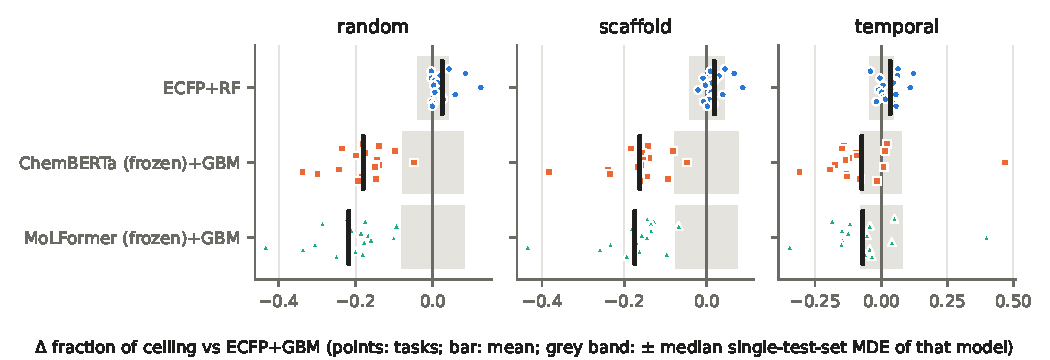
\includegraphics[width=\linewidth]{figures/paired_diff.pdf}
\caption{Per-task difference in fraction of ceiling relative to ECFP+GBM (points: tasks; bar: mean over tasks; grey band: $\pm$ median single-test-set MDE of each model).}\label{fig:paired}\end{figure}

\begin{figure}[ht]\centering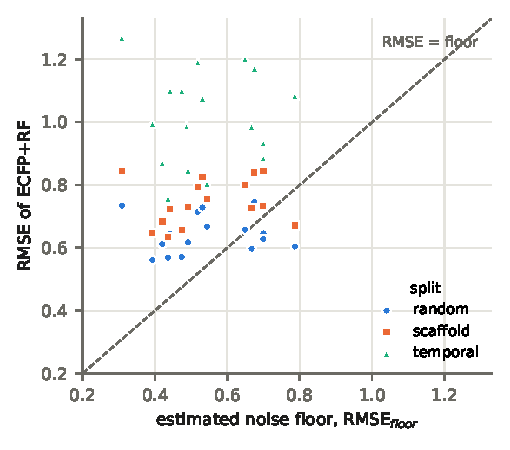
\includegraphics[width=0.5\linewidth]{figures/floor_vs_rmse.pdf}
\caption{Estimated noise floor versus test RMSE of ECFP+RF per task and split. Points below the dashed line have RMSE below the estimated floor ($f>1$).}\label{fig:floor}\end{figure}

\begin{table}[ht]\centering\small\setlength{\tabcolsep}{4pt}\caption{Mean fraction of ceiling $f$ over tasks ($n$ = number of tasks), decontaminated data. Models with $n<17$ were run on a subset of tasks and are not comparable with the rest (see Table~\ref{tab:subset}).}\label{tab:frac}
\begin{tabular}{lcccc}\toprule Model & $n$ & Random & Scaffold & Temporal\\\midrule
ECFP+GBM & 17 & 0.87 & 0.71 & 0.32\\
ECFP+RF & 17 & 0.90 & 0.73 & 0.36\\
ECFP+MLP & 17 & 0.47 & 0.18 & -0.51\\
ChemBERTa-77M (frozen)+GBM & 17 & 0.69 & 0.55 & 0.25\\
MoLFormer-XL-10\% (frozen)+GBM & 17 & 0.66 & 0.54 & 0.25\\
D-MPNN & 5 & 0.63 & 0.54 & 0.27\\
ChemBERTa-77M (fine-tuned) & 5 & 0.60 & 0.49 & 0.31\\
\bottomrule\end{tabular}\end{table}

\begin{table}[ht]\centering\small\setlength{\tabcolsep}{4pt}\caption{Paired difference in $f$ versus ECFP+GBM over 17 tasks (positive = better than ECFP+GBM); Wilcoxon signed-rank test, Holm-adjusted $p$.}\label{tab:paired}
\begin{tabular}{llccc}\toprule Model & Split & mean diff. & better on & $p_{\text{Holm}}$\\\midrule
ECFP+RF & random & +0.024 & 13/17 & 0.013\\
ECFP+RF & scaffold & +0.019 & 13/17 & 0.033\\
ECFP+RF & temporal & +0.034 & 13/17 & 0.032\\
ECFP+MLP & random & -0.400 & 0/17 & $<$0.001\\
ECFP+MLP & scaffold & -0.535 & 0/17 & $<$0.001\\
ECFP+MLP & temporal & -0.836 & 0/17 & $<$0.001\\
ChemBERTa-77M (frozen)+GBM & random & -0.181 & 0/17 & $<$0.001\\
ChemBERTa-77M (frozen)+GBM & scaffold & -0.163 & 0/17 & $<$0.001\\
ChemBERTa-77M (frozen)+GBM & temporal & -0.074 & 4/17 & 0.033\\
MoLFormer-XL-10\% (frozen)+GBM & random & -0.218 & 0/17 & $<$0.001\\
MoLFormer-XL-10\% (frozen)+GBM & scaffold & -0.175 & 0/17 & $<$0.001\\
MoLFormer-XL-10\% (frozen)+GBM & temporal & -0.070 & 3/17 & 0.033\\
\bottomrule\end{tabular}\end{table}

\begin{table}[ht]\centering\small\setlength{\tabcolsep}{4pt}\caption{Mean $f$ on the 5 tasks where D-MPNN (3 seeds) and fine-tuned ChemBERTa (3--5 seeds) were run (CHEMBL204\_Ki, CHEMBL206\_IC50, CHEMBL214\_Ki, CHEMBL237\_IC50, CHEMBL237\_Ki); all models on the same tasks.}\label{tab:subset}
\begin{tabular}{lccc}\toprule Model & Random & Scaffold & Temporal\\\midrule
ECFP+GBM & 0.73 & 0.61 & 0.25\\
ECFP+RF & 0.76 & 0.63 & 0.28\\
ECFP+MLP & 0.36 & 0.07 & -0.41\\
ChemBERTa-77M (frozen)+GBM & 0.61 & 0.49 & 0.27\\
MoLFormer-XL-10\% (frozen)+GBM & 0.58 & 0.47 & 0.23\\
D-MPNN & 0.63 & 0.54 & 0.27\\
ChemBERTa-77M (fine-tuned) & 0.60 & 0.49 & 0.31\\
\bottomrule\end{tabular}\end{table}

\begin{table}[ht]\centering\small\setlength{\tabcolsep}{4pt}\caption{Effect of decontamination: mean $f$ on decontaminated and uncleaned data and mean change in test RMSE (uncleaned $-$ decontaminated) over 17 tasks.}\label{tab:leak}
\begin{tabular}{llccc}\toprule Model & Split & $f$ clean & $f$ uncleaned & $\Delta$RMSE\\\midrule
ECFP+GBM & random & 0.87 & 0.90 & +0.000\\
ECFP+GBM & scaffold & 0.71 & 0.74 & -0.005\\
ECFP+GBM & temporal & 0.32 & 0.35 & -0.003\\
ECFP+RF & random & 0.90 & 0.92 & +0.002\\
ECFP+RF & scaffold & 0.73 & 0.75 & +0.000\\
ECFP+RF & temporal & 0.36 & 0.38 & -0.005\\
ECFP+MLP & random & 0.47 & 0.47 & +0.009\\
ECFP+MLP & scaffold & 0.18 & 0.15 & +0.022\\
ECFP+MLP & temporal & -0.51 & -0.47 & -0.025\\
ChemBERTa-77M (frozen)+GBM & random & 0.69 & 0.71 & +0.006\\
ChemBERTa-77M (frozen)+GBM & scaffold & 0.55 & 0.56 & +0.005\\
ChemBERTa-77M (frozen)+GBM & temporal & 0.25 & 0.26 & +0.004\\
MoLFormer-XL-10\% (frozen)+GBM & random & 0.66 & 0.67 & +0.005\\
MoLFormer-XL-10\% (frozen)+GBM & scaffold & 0.54 & 0.55 & -0.000\\
MoLFormer-XL-10\% (frozen)+GBM & temporal & 0.25 & 0.27 & -0.002\\
\bottomrule\end{tabular}\end{table}
